\chapter{Implementation}\label{chapter:implementation}

In this section different terminology is used, instead of Bob, owner is used,
and instead of Alice sender is used. The implementation of this study is
separated into 3 modules (depicted in \ref{fig:component-diagram}), module for the
circuit which will compute ownership proofs, another one for smart contracts
needed to implement stealth wallet with ZKP stealth address schema, and
module with a web app wallet client used to interact with the stealth wallets.

The implementation is only a proof of concept, not a full featured wallet.
The sender's part is the same as described until now. The owner however,
can only withdraw all funds from the wallet into another address. This does
not detract from demonstrating the core concept of a ZKP stealth address schema.
Fractional withdrawals, ERC20 token transfers, transaction proxying and other wallet
features can be implemented in future work.

\begin{figure}[h!]
    \centering
    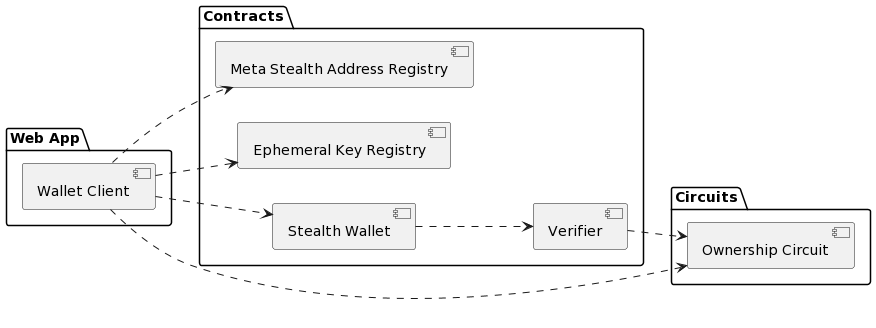
\includegraphics[width=\textwidth]{assets/images/component-diagram.png}
    \caption{Component diagram}
    \label{fig:component-diagram}
    \vspace{0.5cm}
\end{figure}

\section{Requirements}

As mentioned earlier, the implementation is not meant for a full featured wallet,
only a proof of concept one and these are the requirements:

\subsection*{Functional requirements}
\begin{itemize}
    \item \textbf{Meta Stealth Address Retrieval:} The system must enable senders
        to query and retrieve meta stealth addresses from the registry.
    \item \textbf{Ephemeral Key Exchange:} The system needs a mechanism for senders
        to submit ephemeral keys and owners to query them.
    \item \textbf{Stealth Wallet Deployment:} Senders must be able to deploy
        stealth wallet smart contracts, specifying the code and depositing funds.
    \item \textbf{Zero-Knowledge Proof Generation:} The system must provide a way
        for owners to generate Zero-Knowledge Proofs (ZKPs) that demonstrate
        ownership.
    \item \textbf{Zero-Knowledge Proof Verification:} Smart contracts must be able
        to verify the ZKPs submitted by owners.
    \item \textbf{Stealth Wallet Withdrawal:} Upon successful ZKP
        verification, the smart contract must execute a withdrawal, transferring
        the entire stealth wallet balance to the owner's designated address.
\end{itemize}

\subsection*{Non-functional requirements}
\begin{itemize}
    \item \textbf{Security:} The system must prioritize the protection of private keys.
    \item \textbf{Privacy:} Stealth addresses and the link between owners and
        their stealth wallets should be obscured to preserve on-chain privacy.
    \item \textbf{Compatibility:} The system should be compatible with
        relevant Ethereum testnet environment, not only a local
        development environment.
\end{itemize}

\pagebreak
\section{Interaction between components}

The interaction between components, and users is depicted in Figure \ref{fig:component-diagram}.

\begin{figure}[h!]
    \centering
    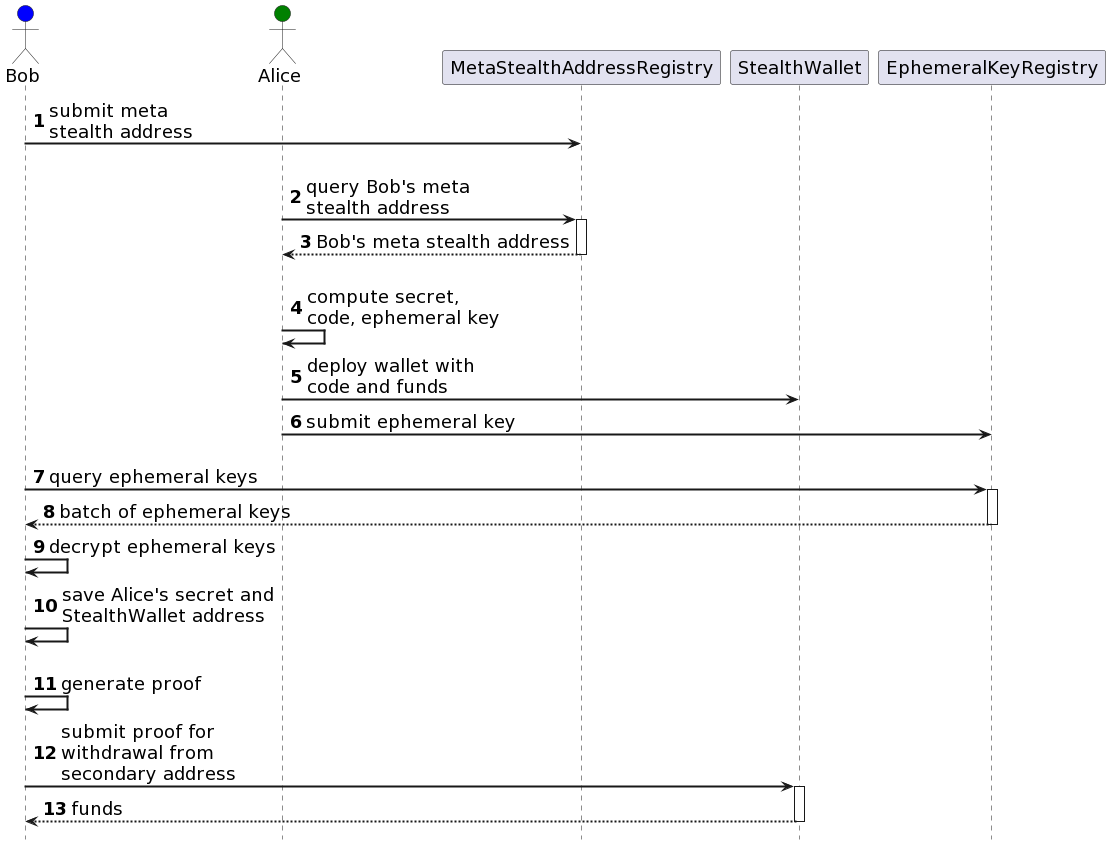
\includegraphics[width=\textwidth]{assets/images/implementation-flow.png}
    \caption{Component diagram}
    \label{fig:implementation-diagram}
    \vspace{0.5cm}
\end{figure}


\section{Circuits}

Circuits for proving and verifying ZKPs are written in Circom 2\cite{circomCircomDocumentation}.
With circom compiler, a circuit is compiled into a Groth16
ZK-SNARK proof system\cite{Groth16} representation. Circom also generates
either C++ of Wasm source files for computing witness (proof) for the
circuit. Circuit written in this study, which proves ownership, has
these private inputs:
\begin{enumerate}
    \item owner's secret value,
    \item sender's secret value,
    \item and the withdrawee address.
\end{enumerate}
And these public inputs:
\begin{enumerate}
    \item code that was submitted by sender on contract creation,
    \item and the transaction sender.
\end{enumerate}

Groth16 requires a trusted setup for each circuit. For Groth16 trusted
setup, there are two parts:
\begin{enumerate}
    \item Powers of Tau ceremony\cite{PowersOfTau},
    \item and phase 2 dependent on the circuit.
\end{enumerate}
Powers of Tau ceremony is used to generate initial parameters for a SNARK.
In this ceremony, the initial parameters are generated using a multi-party
computation. If only one party in this computation is acting honestly,
the entire process is trustworthy and the initial parameters are secure
for use with any circuit. There is ongoing public powers of tau ceremony
called Perpetual Powers of Tau \cite{PerpetualPTAU}. Its goal is to
securely generate SNARK parameters for circuits. In this study a powers
of tau ceremony file from SnarkJS\cite{snarkjs} is used, which is from
this ceremony. Phase 2 is generated with SnarkJS and is specific for circuit.

\section{Smart contracts}

Smart contracts in this implementation are written in programming
language Solidity\cite{solidity} and are developed and tested
with Foundry\cite{foundry}. They are deployed through
Infura\cite{infura} Ethereum RPC provider to the Sepolia Ethereum
testnet\cite{sepolia}.

There are four smart contracts implemented. A meta stealth address
registry which holds meta stealth addresses. A ephemeral key registry
which holds the ephemeral keys. A verifier of previously mentioned
circuit. And contract for the stealth wallet.

Owners submit their meta stealth addresses to meta stealth address registry,
and senders query it for them. To the ephemeral key registry senders submit
ephemeral keys and owners query it for them. Senders deploy stealth wallets
with funds and computed codes. Owners send proofs to stealth wallets,
which interact with the verifier.

This module also contains tests. Code coverage report for these is shown in
table \ref{table:coverage}.

\begin{table}[ht]
\centering
\scalebox{0.7}{
    \begin{tabular}{l | r r r r}
    \toprule
        \textbf{File} & \textbf{\% Lines} & \textbf{\% Statements}  & \textbf{\% Branches}  & \textbf{\% Funcs} \\ 
        \midrule
        script/DeployConfig.s.sol  & 0.00\% (0/5)    & 0.00\% (0/7)     & 0.00\% (0/2)     & 0.00\% (0/3)   \\
        script/DeployContracts.s.sol & 0.00\% (0/7)    & 0.00\% (0/9)     & 100.00\% (0/0)   & 0.00\% (0/1)   \\
        src/EphemeralKeyRegistry.sol & 92.86\% (13/14) & 94.44\% (17/18)  & 66.67\% (4/6)    & 66.67\% (2/3)  \\
        src/MetaStealthAddressRegistry.sol & 100.00\% (8/8)  & 100.00\% (11/11) & 100.00\% (4/4)   & 100.00\% (2/2) \\ 
        src/StealthWallet.sol  & 91.67\% (11/12) & 92.31\% (12/13)  & 83.33\% (5/6)    & 66.67\% (2/3)  \\
        src/Verifier.sol   & 100.00\% (0/0)  & 100.00\% (0/0)   & 100.00\% (0/0)   & 100.00\% (1/1) \\
        \midrule
        \textbf{Total} & 69.57\% (32/46) & 68.97\% (40/58)  & 72.22\% (13/18)  & 53.85\% (7/13) \\
        \bottomrule
        \end{tabular}
}
\caption{Solidity code coverage}
\label{table:coverage}
\end{table}

The first two files are not covered, because they only contain simple logic
for deploying contracts and do not interfere in any functionality of the
implemented stealth address scheme.

\section{Web app}

Browser wallet client used to interact with stealth wallets is written in
frontend framework SolidJS\cite{solidjs}, with Web3JS\cite{web3js}
as the main library for interacting with blockchain, and Infura\cite{infura}
is used as a Ethereum RPC provider.

It consists of two sub-pages, one for sender (Alice), in which a sender
can query meta stealth addresses and deploy stealth wallets only accessible
by the owners of corresponding meta stealth addresses. And the second one,
for owners (Bob) which displays all stealth wallets with balance and enables
owners to withdraw funds from them by generating ZKPs.

